\section{5. Documentation, Reports, Slides, and Publication
Paths}\label{documentation-reports-slides-and-publication-paths}

This section maps the repo's explanatory material so readers can see
which document family answers which type of question.

\subsection{5.1 Onboarding and specification
material}\label{onboarding-and-specification-material}

This subsection groups the documents that explain the project cleanly
before a reader needs the report library.

Two document clusters matter most here.
\href{https://github.com/chris-page-gov/mcp-geo/blob/fe862910da246ca77f374cfbe484985f5df4d316/docs/getting_started.md}{docs/getting\_started.md}
and the
\href{https://github.com/chris-page-gov/mcp-geo/blob/fe862910da246ca77f374cfbe484985f5df4d316/README.md\#L20-L240}{root
README} explain usage and setup, while the
\href{https://github.com/chris-page-gov/mcp-geo/tree/fe862910da246ca77f374cfbe484985f5df4d316/docs/spec_package}{spec
package} gives the test-ready design view through
\href{https://github.com/chris-page-gov/mcp-geo/blob/fe862910da246ca77f374cfbe484985f5df4d316/docs/spec_package/03_architecture.md}{architecture},
\href{https://github.com/chris-page-gov/mcp-geo/blob/fe862910da246ca77f374cfbe484985f5df4d316/docs/spec_package/06_api_contracts.md}{API
contracts},
\href{https://github.com/chris-page-gov/mcp-geo/blob/fe862910da246ca77f374cfbe484985f5df4d316/docs/spec_package/07_security_privacy.md}{security
and privacy}, and
\href{https://github.com/chris-page-gov/mcp-geo/blob/fe862910da246ca77f374cfbe484985f5df4d316/docs/spec_package/09_testing_quality.md}{testing
and quality}. Open these first when the question is ``What is the
intended design?'' rather than ``What happened in a specific
experiment?''.

Where to go:
\href{https://github.com/chris-page-gov/mcp-geo/blob/fe862910da246ca77f374cfbe484985f5df4d316/docs/getting_started.md}{docs/getting\_started.md},
\href{https://github.com/chris-page-gov/mcp-geo/blob/fe862910da246ca77f374cfbe484985f5df4d316/docs/spec_package/README.md\#L1-L45}{docs/spec\_package/README.md},
\href{https://github.com/chris-page-gov/mcp-geo/blob/fe862910da246ca77f374cfbe484985f5df4d316/docs/spec_package/03_architecture.md}{docs/spec\_package/03\_architecture.md},
\href{https://github.com/chris-page-gov/mcp-geo/blob/fe862910da246ca77f374cfbe484985f5df4d316/docs/spec_package/06_api_contracts.md}{docs/spec\_package/06\_api\_contracts.md},
and
\href{https://github.com/chris-page-gov/mcp-geo/blob/fe862910da246ca77f374cfbe484985f5df4d316/docs/spec_package/09_testing_quality.md}{docs/spec\_package/09\_testing\_quality.md}.

\subsection{5.2 Community narrative, reports, and slide
assets}\label{community-narrative-reports-and-slide-assets}

This subsection explains where the repo stops being purely technical and
becomes a narrative record of delivery, evaluation, and public
communication.

The most approachable narrative path is the
\href{https://github.com/chris-page-gov/mcp-geo/tree/fe862910da246ca77f374cfbe484985f5df4d316/docs/public_sector_ai_community}{community
documentation set}, whose
\href{https://github.com/chris-page-gov/mcp-geo/blob/fe862910da246ca77f374cfbe484985f5df4d316/docs/public_sector_ai_community/README.md\#L1-L60}{README}
explains its audience and scope boundaries. The dense evidence surface
sits next to it in the
\href{https://github.com/chris-page-gov/mcp-geo/blob/fe862910da246ca77f374cfbe484985f5df4d316/docs/reports/README.md\#L1-L71}{report
library}, while the talk itself is represented by the
\href{https://github.com/chris-page-gov/mcp-geo/blob/fe862910da246ca77f374cfbe484985f5df4d316/docs/slides/20260225\%20-\%20From_Apps_to_Answers.pdf}{slide
deck} and the
\href{https://github.com/chris-page-gov/mcp-geo/blob/fe862910da246ca77f374cfbe484985f5df4d316/docs/reports/mcp_geo_ai_community_event_record.docx}{event
record DOCX}. Read this cluster when the task is to understand how the
repo has been communicated and evidenced publicly.

Where to go:
\href{https://github.com/chris-page-gov/mcp-geo/blob/fe862910da246ca77f374cfbe484985f5df4d316/docs/public_sector_ai_community/README.md\#L1-L60}{docs/public\_sector\_ai\_community/README.md},
\href{https://github.com/chris-page-gov/mcp-geo/blob/fe862910da246ca77f374cfbe484985f5df4d316/docs/reports/README.md\#L1-L71}{docs/reports/README.md},
\href{https://github.com/chris-page-gov/mcp-geo/tree/fe862910da246ca77f374cfbe484985f5df4d316/docs/slides}{slides
directory}, and
\href{https://github.com/chris-page-gov/mcp-geo/blob/fe862910da246ca77f374cfbe484985f5df4d316/docs/reports/mcp_geo_ai_community_event_record.docx}{event
record DOCX}.

\begin{figure}
\centering
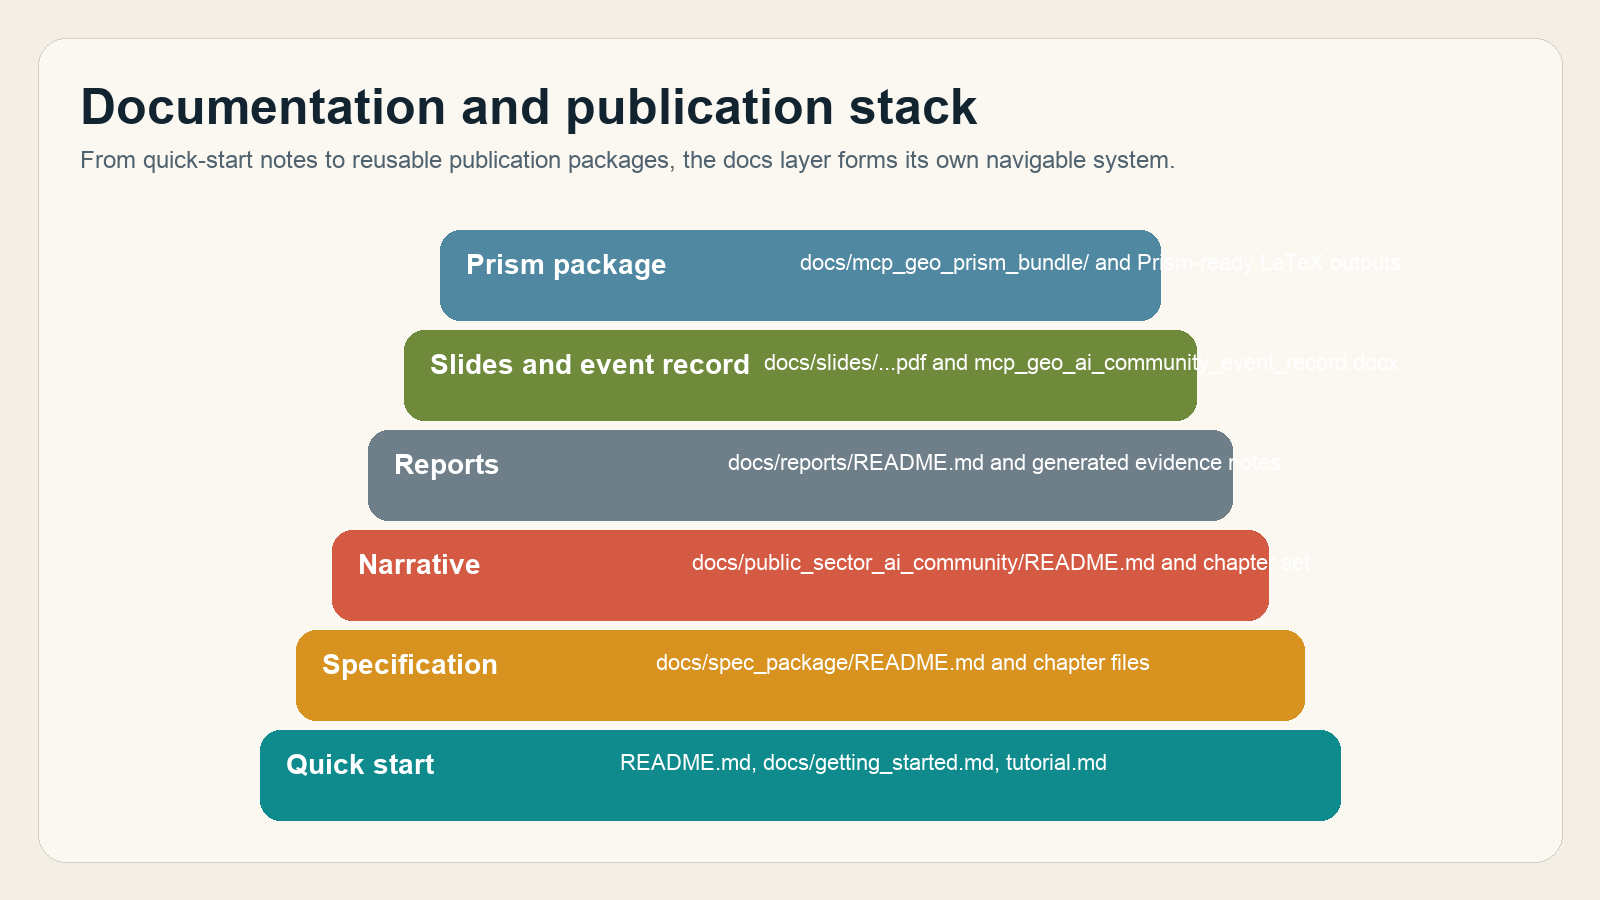
\includegraphics[width=0.96\linewidth,height=\textheight,keepaspectratio,alt={Figure F05. Documentation and publication stack}]{figures/f05_documentation_publication_stack.png}
\caption{Figure F05. Documentation and publication stack}
\end{figure}

Figure F05 shows the publication ladder from setup docs to full
publication bundles instead of treating every document as equal.

\subsection{5.3 Prism and publication
stack}\label{prism-and-publication-stack}

This subsection shows where publication-ready packaging already exists
and where this replacement index now sits inside that stack.

The earlier public-facing Prism precedent is the
\href{https://github.com/chris-page-gov/mcp-geo/tree/fe862910da246ca77f374cfbe484985f5df4d316/docs/public_sector_ai_community/prism}{community
documentation Prism package}, whose
\href{https://github.com/chris-page-gov/mcp-geo/blob/fe862910da246ca77f374cfbe484985f5df4d316/docs/public_sector_ai_community/prism/main.tex\#L1-L35}{main.tex}
and
\href{https://github.com/chris-page-gov/mcp-geo/blob/fe862910da246ca77f374cfbe484985f5df4d316/docs/public_sector_ai_community/prism/README.md\#L1-L16}{README}
show the expected structure. The rough initial Analytical Index attempt
lived in
\href{https://github.com/chris-page-gov/mcp-geo/blob/fe862910da246ca77f374cfbe484985f5df4d316/docs/mcp_geo_prism_bundle/main.md\#L1-L292}{docs/mcp\_geo\_prism\_bundle/main.md};
this replacement now occupies the same bundle path with a repeatable
Markdown-first workflow and a stronger figure-prompt appendix.

Where to go:
\href{https://github.com/chris-page-gov/mcp-geo/tree/fe862910da246ca77f374cfbe484985f5df4d316/docs/public_sector_ai_community/prism}{community
Prism package},
\href{https://github.com/chris-page-gov/mcp-geo/blob/fe862910da246ca77f374cfbe484985f5df4d316/docs/public_sector_ai_community/prism/main.tex\#L1-L35}{community
Prism \texttt{main.tex}},
\href{https://github.com/chris-page-gov/mcp-geo/blob/fe862910da246ca77f374cfbe484985f5df4d316/docs/mcp_geo_prism_bundle/main.md\#L122-L292}{rough
analytical-index baseline}, and
\href{https://github.com/chris-page-gov/mcp-geo/tree/fe862910da246ca77f374cfbe484985f5df4d316/docs/mcp_geo_prism_bundle}{current
bundle directory}.

\begin{figure}
\centering
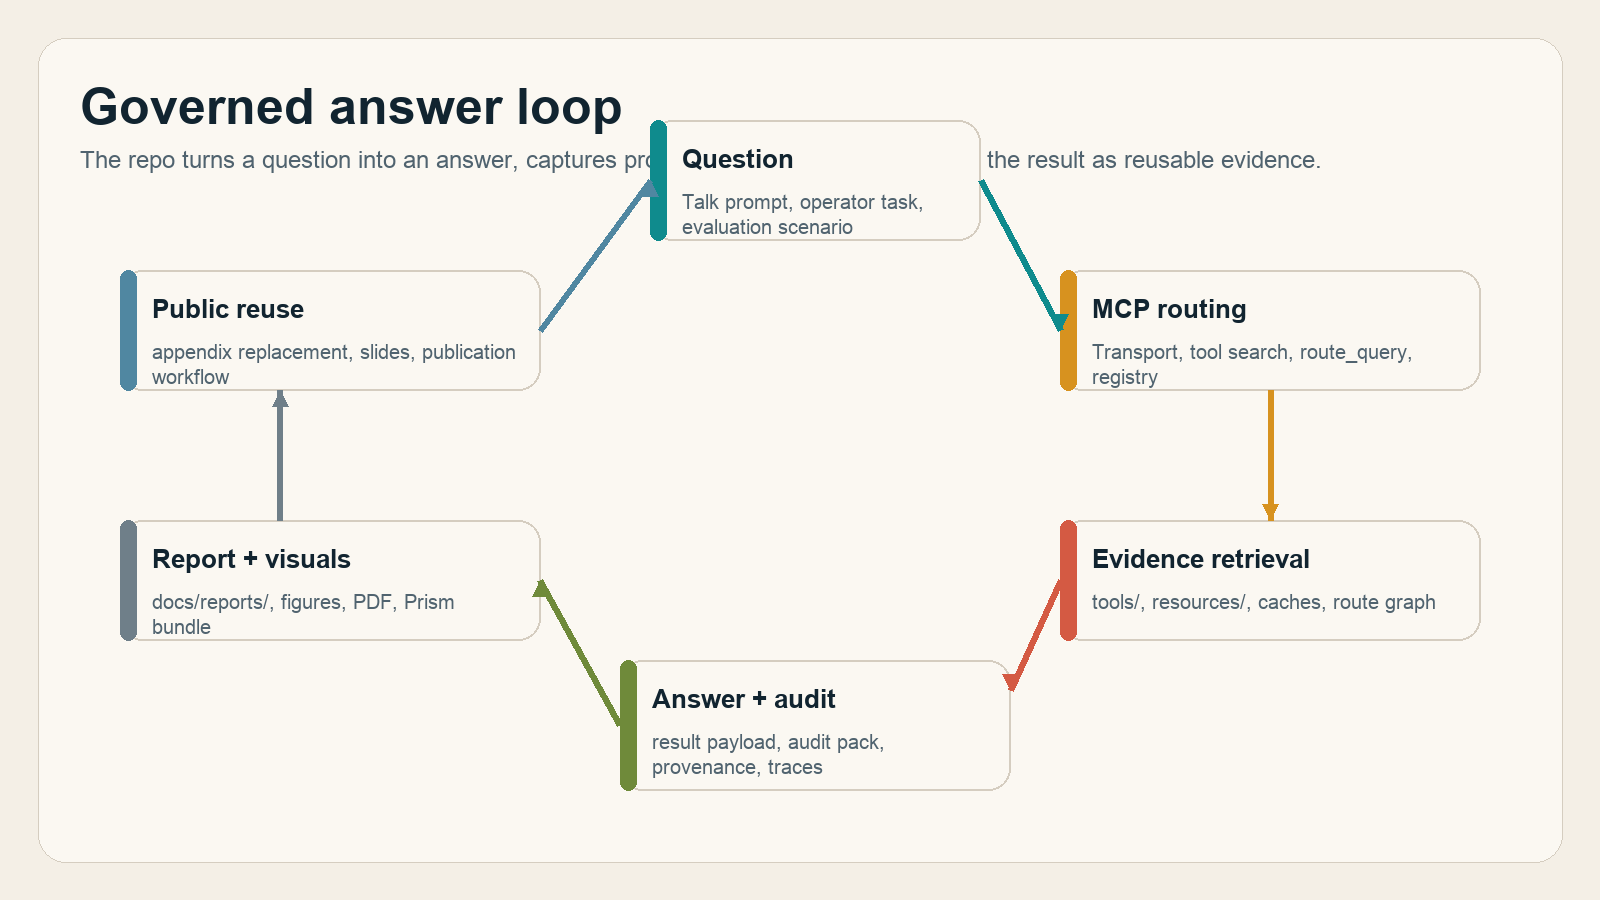
\includegraphics[width=0.96\linewidth,height=\textheight,keepaspectratio,alt={Figure F08. Governed answer loop}]{figures/f08_governed_answer_loop.png}
\caption{Figure F08. Governed answer loop}
\end{figure}

Figure F08 ties the talk thesis back to the repo by showing how a
question becomes an inspectable answer and then a publication artifact.
